We have extensively studied parameteric supervised models like linear regression, SVMs, and softmax regression. Now we introduce analogues in the nonparameteric scheme, starting with kernel regression. If all data was intrinsically linear, then this would be an ideal world where we only need linear regression. However, this is not the case in reality, and we must resort to more flexible models to fit nonlinear data. 

The basic motivation behind kernels is that samples with similar covariates $x_1, \ldots, x_d$ should be similar in their response $y$. Therefore, two data points $x^{(1)}, x^{(2)}$ near each other should have similar $y^{(1)}, y^{(2)}$ and so if we are given a new sample $x^{(n+1)}$, we should use similar samples to predict the corresponding $y^{(n+1)}$. 

Like with a lot of things, we can in fact formalize this by constructing \textit{reproducing kernel Hilbert spaces (RKHS)}. RKHS regression provides the theoretical foundation that explains why many kernel methods work. The representer theorem shows that solutions to regularized regression problems in an RKHS can be expressed as linear combinations of kernel functions evaluated at nearby training points. 

One thing to keep in mind for nonparameteric classification is that when you are using plug-in classifiers (train a regressor and then run it through a threshold function), there may be problems near the boundary. For example, say that in a one-dimensional case, you would want the regressor to smoothly fit across the decision boundary. Classification could be difficult if we have bad boundaries, but the good news is that if the probability that the data lies in the margins is not high, then we can do pretty well in classification. 

\begin{figure}[H]
  \centering
  \begin{subfigure}[b]{0.48\textwidth}
    \centering
    \begin{tikzpicture}[scale=0.7]
      \begin{axis}[
        axis lines = center,
        xlabel = {$x$},
        ylabel = {$y$},
        domain = -6:6,
        samples = 100,
        grid = major,
        xmin = -6, xmax = 6,
        ymin = -0.2, ymax = 1.2,
        width = 10cm,
        height = 8cm,
        xtick = \empty,
        ytick = {0, 0.5, 1}
      ]
     
        % Sigmoid function
        \addplot[blue, thick] {1/(1+exp(-x))};
     
        % Horizontal line at y = 1/2
        \addplot[red, thick] {0.5};
     
      \end{axis}
    \end{tikzpicture}
    \caption{Good case.}
  \end{subfigure}
  \hfill 
  \begin{subfigure}[b]{0.48\textwidth}
    \centering
    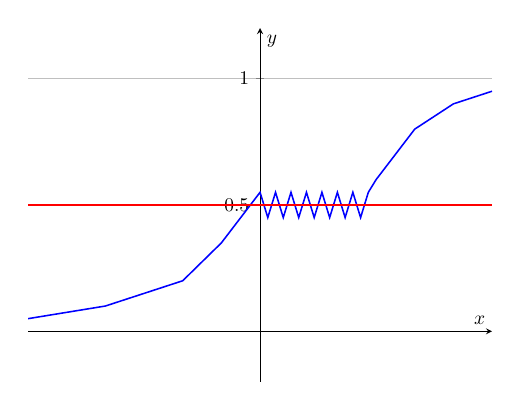
\begin{tikzpicture}[scale=0.7]
      \begin{axis}[
        axis lines = center,
        xlabel = {$x$},
        ylabel = {$y$},
        domain = -6:6,
        grid = major,
        xmin = -6, xmax = 6,
        ymin = -0.2, ymax = 1.2,
        width = 10cm,
        height = 8cm,
        xtick = \empty,
        ytick = {0, 0.5, 1}
      ]
     
        % Function drawn by connecting points
        \addplot[blue, thick] coordinates {
          (-6, 0.05)
          (-4, 0.1)
          (-2, 0.2)
          (-1, 0.35)
          (-0.5, 0.45)
          (0, 0.55)
          (0.2, 0.45)
          (0.4, 0.55)
          (0.6, 0.45)
          (0.8, 0.55)
          (1.0, 0.45)
          (1.2, 0.55)
          (1.4, 0.45)
          (1.6, 0.55)
          (1.8, 0.45)
          (2.0, 0.55)
          (2.2, 0.45)
          (2.4, 0.55)
          (2.6, 0.45)
          (2.8, 0.55)
          (3.0, 0.6)
          (3.5, 0.7)
          (4, 0.8)
          (5, 0.9)
          (6, 0.95)
        };
     
        % Horizontal line at y = 1/2
        \addplot[red, thick] {0.5};
     
      \end{axis}
    \end{tikzpicture}
    \caption{Bad case.}
  \end{subfigure}
  \caption{We will generally have challenges differentiating points at the boundaries of a plug-in classifier. This may matter if $p(x, y)$ is concentrated around this jagged region, or it may not if most of the masses are concentrated far away from the boundary.}
\end{figure}


